\section{Apparato Sperimentale}



\subsection{Parabola}
Lo strumento utilizzato per la ricezione del segnale è un telescopio riflettore, ovvero un'antenna radio di forma parabolica, il cui diametro è di 3 m. Nel punto focale sono situati i ricevitori, tre analogici e uno digitale.
I ricevitori analogici lavorano a diverse frequenze, 1,4; 2,5; 10 GHz. A sua volta il ricevitore digitale presenta due porte di ingresso, una a 1,4 GHz e una a 2,5 GHz.
In particolare, nella seguente analisi verrà utilizzato la porta a 1,4 GHz del ricevitore digitale.
\\\\
Per muovere la parabola nella regione di cielo di interesse, vengono inseriti, sul software, i valori di azimuth, elevazione e orario di puntamento. Per quanto concerne l'azimuth, è da tener conto l'off-set dovuto alla posizione del ricevitore. Nel caso in esame l'off-set corrisponde ad un angolo di 21.0 gradi. 

\subsection{Ricevitore digitale}
La larghezza di banda del ricevitore è di 160 MHz, permettendo così un'analisi in un range di $\nu \in$  [1,30;1,46] GHz. Sono presenti 8192 canali, ciascuno con una larghezza di banda pari a $\Delta\nu$ = 19531,25 Hz \cite{Canali:canali}.%non funziona la citazione
\\\\
La velocità di campionamento della radio è di 160 Msamples/s, la media temporale è eseguita su 320 Msamples spaziando un intervallo di circa 2 secondi. Tale media permette di ottenere un dato sufficientemente sensibile a variazioni dell'ordine del secondo, oltre a ridurre sensibilmente il rumore. 


\subsection{Organizzazione file}
Le misure vengono salvate su un unico file dopo aver collezionato 150 record. Ogni file corrisponde a un tempo di presa dati di circa 5 minuti.
\\\\
I file, restituiti dal ricevitore digitale, sono organizzati nella seguente modalità. In ciascun record, i primi tre valori corrispondono rispettivamente a:
\begin{itemize}
\item tempo: tempo trascorso dall'apertura del file espresso in millisecondi;
\item frequenza: frequenza del canale a frequenza più bassa espressa in Hz;
\item frequency step: step in frequenza tra due canali successivi, espresso in Hz.
\end{itemize}
Le entrate successive, espresse in dBm, corrispondono al segnale registrato dal ricevitore, ripetuto per ognuno degli 8192 canali.
\\\\
Nell'analisi sono anche utilizzati i file della parabola, da cui si ricavano i valori di temperatura del cavo che connette la parabola al ricevitore. %capire ricevitore/elaboratore


\subsection{Programma coordinate}
\label{Programma coordinate}
Dato un orario di osservazione, per determinare le coordinate a cui porre la parabola, viene utilizzata la libreria astropy. In particolare la funzione che implementa il cambio di coordinate da celesti ad azimuth ed elevazione è \textit{transform to}.  Necessario conoscere i valori di longitudine, latitudine ed elevazione rispetto al livello del mare del luogo in cui è situata la parabola, i.e. Milano. Inoltre bisogna tener conto della regione UTC, per settare correttamente l'offset. 

\begin{figure}[h]
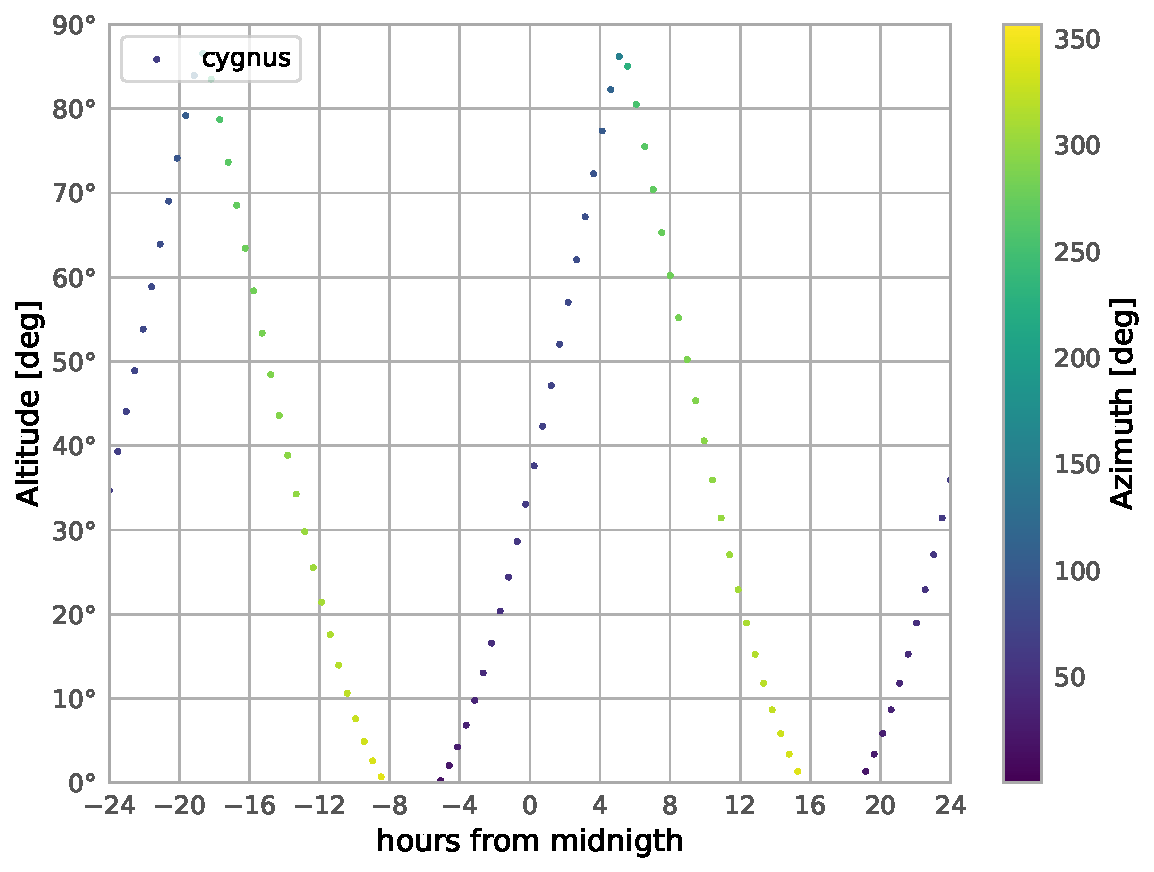
\includegraphics[scale=0.60]{Coordinate.pdf}
\centering
\caption{L'immagine mostra la traiettoria della sorgente in un arco di 48 ore.}
\label{fig:Coordinate}
\end{figure}
